\documentclass[12pt]{article}
\setlength{\headheight}{14.5pt}
\addtolength{\topmargin}{-2.5pt}

\usepackage{pgfplots} % Add this line to include the pgfplots package
\usepackage{amsmath}
\usepackage{geometry}
\usepackage{setspace}
\usepackage{graphicx}
\usepackage{fancyhdr}
\usepackage{xcolor}
\usepackage{titlesec}
\usepackage{booktabs}
\usepackage{hyperref}
\usepackage{soul}
\usepackage{wrapfig}
\usepackage{placeins}
 


\hypersetup{
    colorlinks=true,       % Enable colored links
    linkcolor=blue,        % Color of internal links
    filecolor=magenta,     % Color of file links
    urlcolor=cyan          % Color of external links
}



\renewcommand{\headrulewidth}{0pt} % Remove header rule
\renewcommand{\footrulewidth}{0pt} % Remove footer rule




\usepackage{url}
\geometry{a4paper, margin=1in}
\setlength{\parindent}{0pt}
\setstretch{1.5}
\usepackage{setspace}
% Header and Footer
\usepackage{fancyhdr}
\pagestyle{fancy}
\fancyhf{} % Clear all header and footer fields
\fancyhead[L]{\textbf{19-AIBM4}} % Top-left text
\fancyhead[C]{\rule{\textwidth}{0.5pt}} % Top horizontal line

% Combine the page numbering and horizontal rule into one footer definition
\fancyfoot[C]{\rule{\textwidth}{0.5pt}\\ Page \thepage\ of 15} % Bottom horizontal line with page number


% Title formatting
\titleformat{\section}[block]
  {\large\bfseries\sffamily\color{red}}
  {\thesection.}{1em}{}

\titleformat{\subsection}[block]
  {\normalsize\bfseries\sffamily\color{red}}
  {\thesubsection}{1em}{}
 \pgfplotsset{compat=1.18} 
\begin{document}


\pagenumbering{arabic} % Ensure Arabic numbering starts from the first page


 
% -------------------------------------------------------------
% COVER PAGE
% -------------------------------------------------------------
\begin{titlepage}
\centering
% University logo or other image

\includegraphics[width=0.4\textwidth]{UoD_Engineering.jpg} \\
\vspace{10mm}

% Title and subtitle
{\LARGE \textbf{Feasibility Report for 19-AIBM4 Autonomous Material Mover}} \\[10pt]

\vspace{5mm}\hrule\vspace{0mm}

% Insert image with caption for the material mover
\begin{figure}[h!]
    \centering
     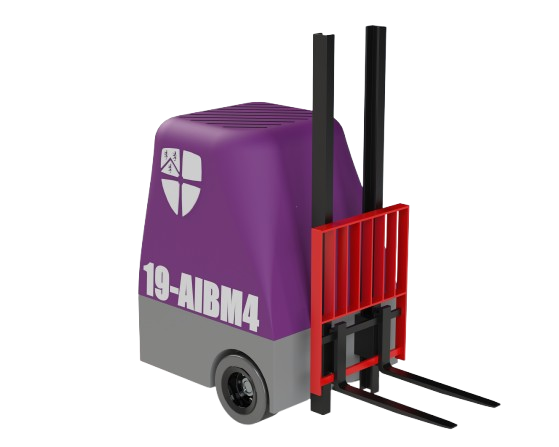
\includegraphics[width=1\textwidth]{Pooled_Design_V2__6_-removebg-preview.png}
\end{figure}  
\vspace{0mm}
\vspace{10mm}

% Title and author block
{\large \textbf{Co-Authors: }\textit{Abi Wright, Anna Wigmore, Henry Billing, Jiaxi Wang, Louis Nangle, William Woodward}} \\ \vspace{1mm}
{Supervisors:\textit{ Aissa Ikhlef, Bill Maxwell}} \\[10pt]
{\small The University of Durham \\ \today}
\end{titlepage}

% -------------------------------------------------------------
% FRONTMATTER
% -------------------------------------------------------------
\tableofcontents
%\begin{figure}[h!]
 %   \centering
 %    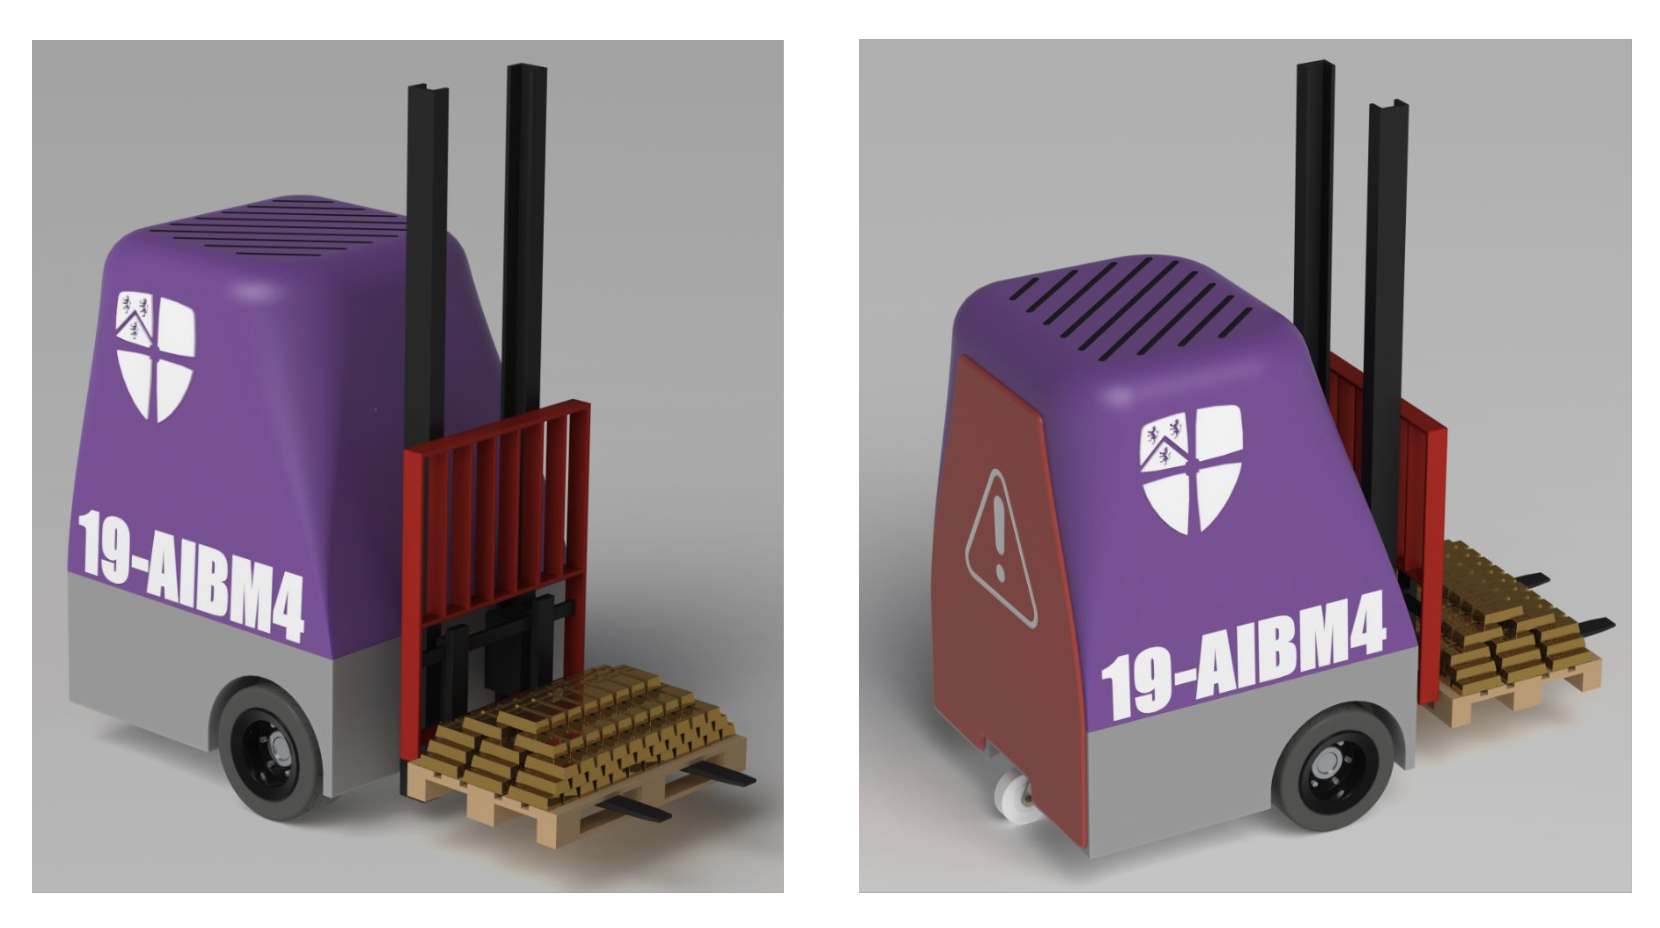
\includegraphics[width=0.65\textwidth]{finaldesign.png}
 %         \label{fig:final design}
%\end{figure}

\newpage

% -------------------------------------------------------------
% MAIN CONTENT
% -------------------------------------------------------------


% -------------------------------------------------------------
% 2. Introduction and Project Scope
% -------------------------------------------------------------
\section{Introduction}
\subsection{Overview}
This feasibility report aims to look into the development of the Automated Material Mover (AIBM4), which aims to transport materials autonomously within a factory environment. This would eliminate the need for manual handling of goods as well as enhancing productivity and ensuring a safer and more sustainable working environment.
\subsection{What is the problem that you’re attempting to solve?}
Efficient material handling is essential in modern manufacturing, but conventional forklifts still require manual operation. This project seeks to eliminate manual dependency by designing an autonomous material mover.
 
\subsection{Issues with Conventional Manual Material Handling}

Manual labour and forklifts have several key issues within factory environments such as:

\begin{itemize}
    \item \textbf{Inefficiency:} Time lost due to the requirements of having human interactions, e.g., lunch breaks are required.
    \item \textbf{Safety concerns:} Human error can lead to an increased likelihood of an accident as well as a higher chance of injuries.
    \item \textbf{Cost:} Labour can be a very expensive cost, and for operations to continue 24 hours a day, this may require three shift workers.
    \item \textbf{Reliability:} Human error can lead to materials being moved to the wrong locations.
\end{itemize}

Overall, these issues reduce productivity and compromise workplace safety.



\begin{figure}[htbp]
\section{Project Scope}
    \centering
     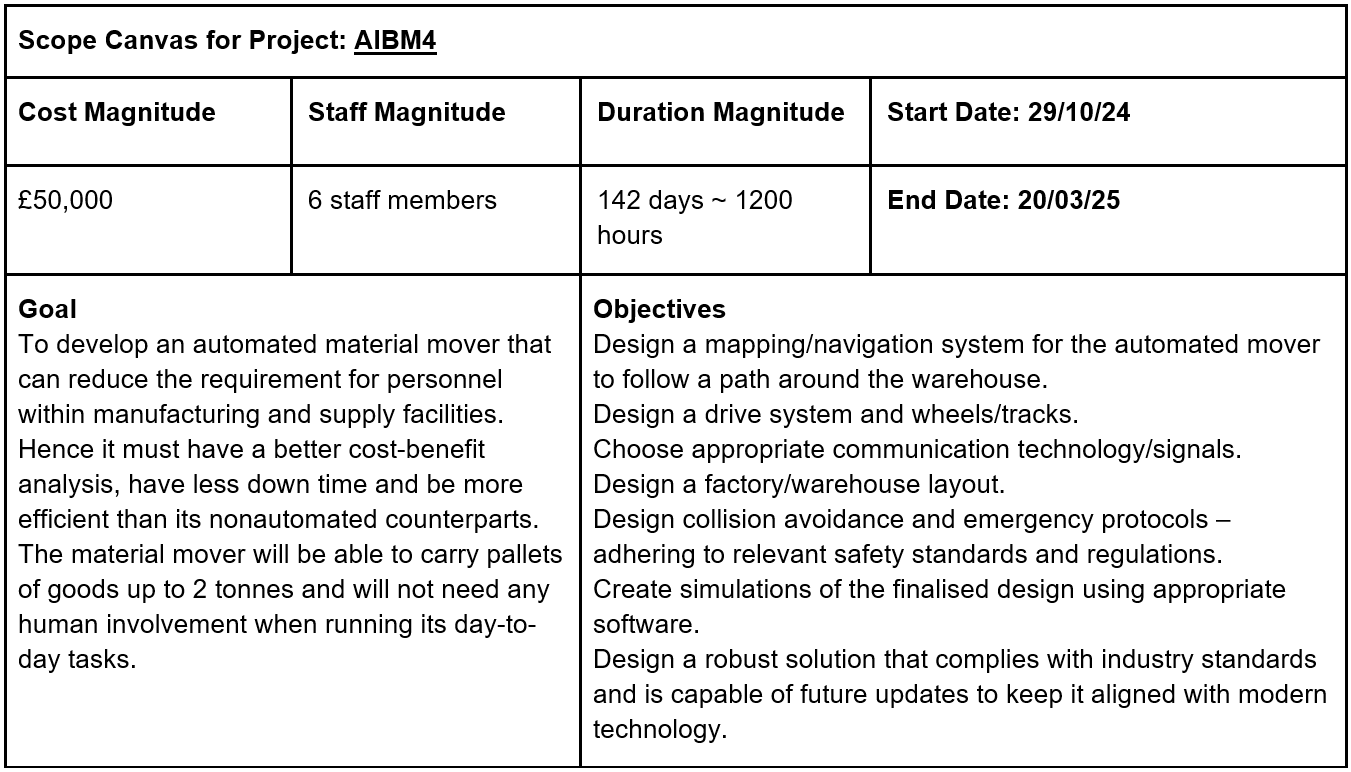
\includegraphics[width=0.9\textwidth]{Scope Canvas 1.png}
     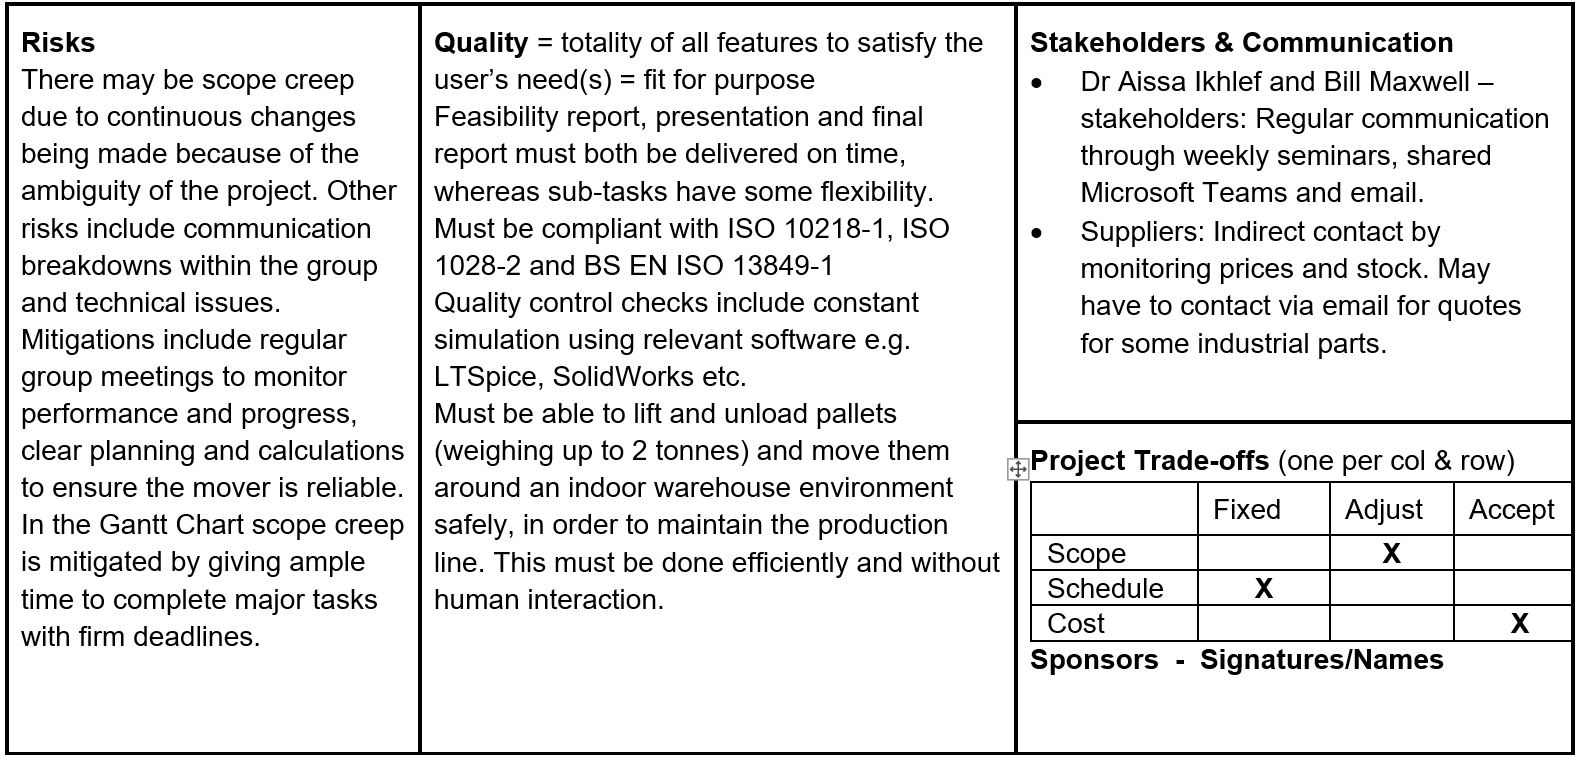
\includegraphics[width=0.9\textwidth]{Scope Canvas 2.png}
     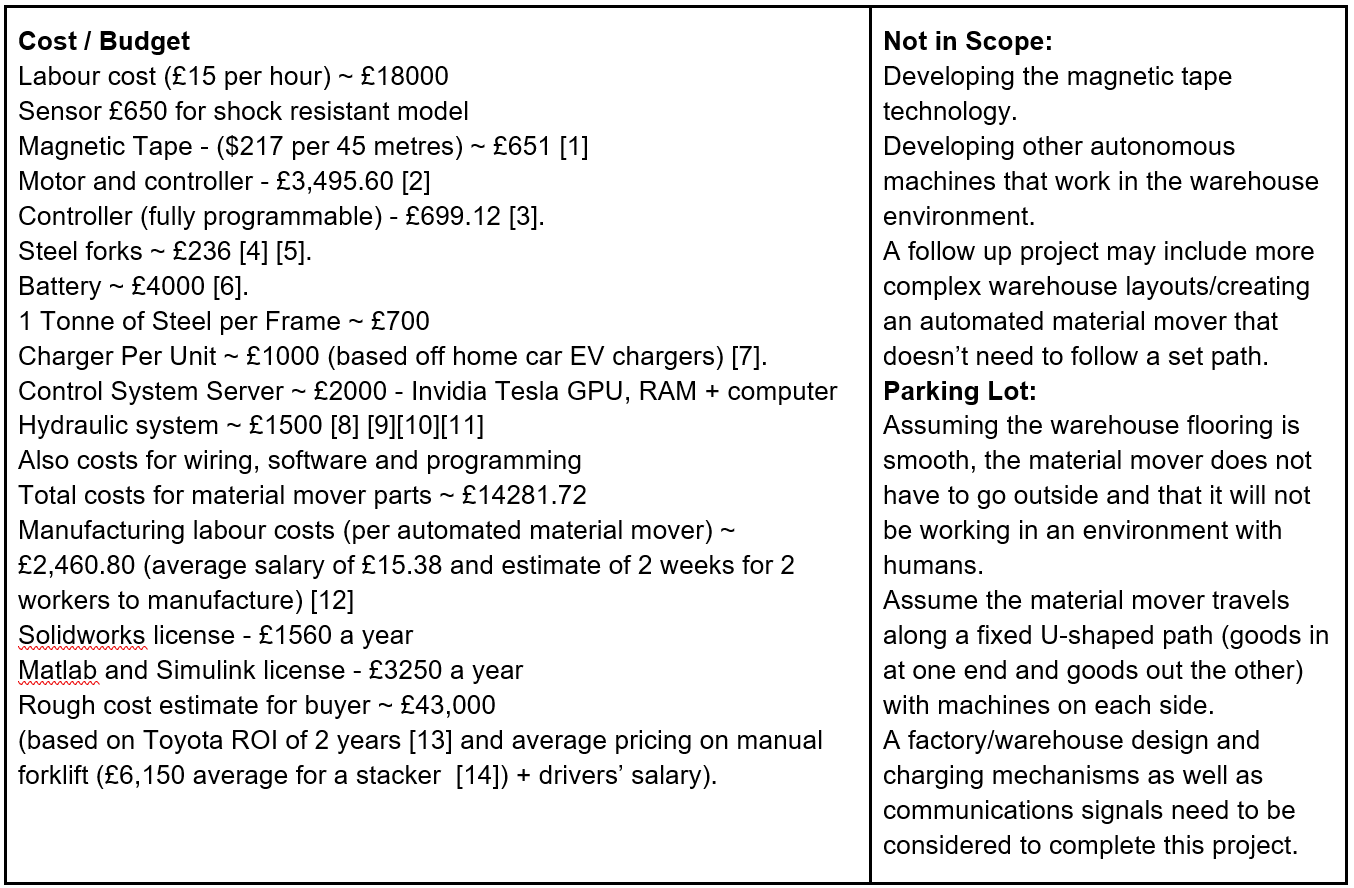
\includegraphics[width=0.9\textwidth]{Scope Canvas 3.png}
   

\end{figure}
\clearpage
\begin{figure}[htbp]

    \centering
     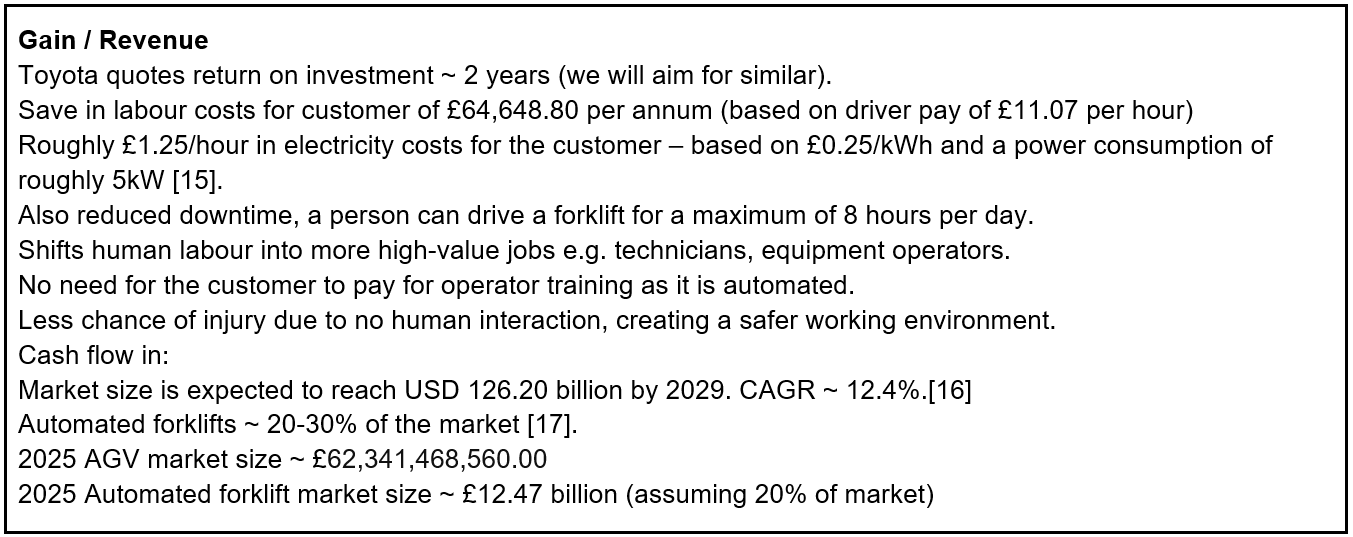
\includegraphics[width=1\textwidth]{Scope Canvas 4.png}
\end{figure}
\FloatBarrier




\begin{figure}[ht]
 
\section{User Requirement Specification (URS)}
    \centering
     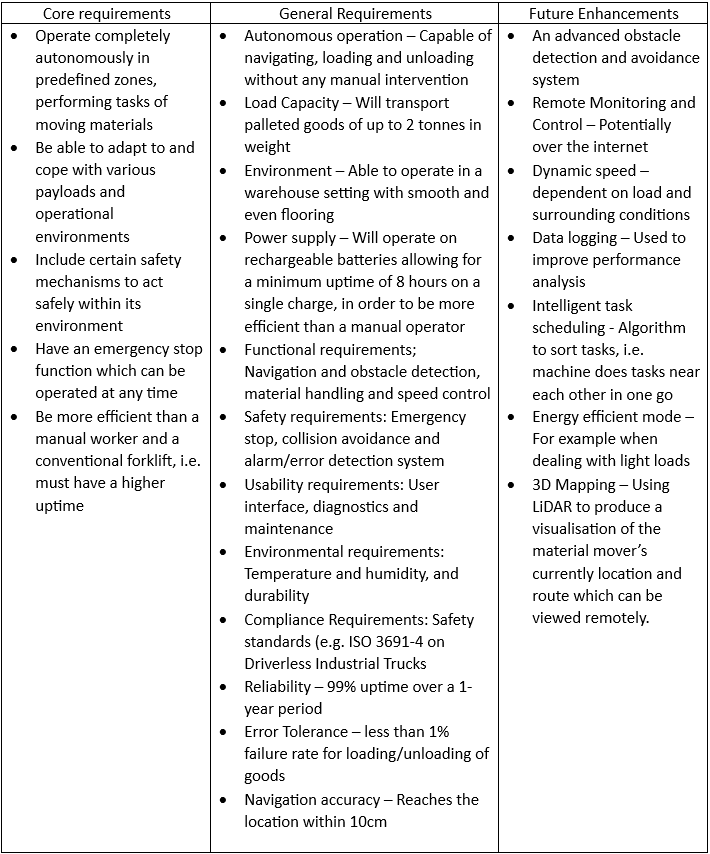
\includegraphics[width=1.05\textwidth]{URS.png}
     \caption{URS – Automated Material Mover Project}
    \label{fig:URS}
\end{figure}
\FloatBarrier

\newpage
% -------------------------------------------------------------
% 3. Concepts
% -------------------------------------------------------------
\section{Concepts}
\subsection{Possible Concepts}
Three design concepts were considered:
\begin{enumerate}
    \item A three-wheeled automated forklift with line-following sensors.
    \item A four-wheeled heavy-duty material mover with obstacle detection.
    \item A hybrid robotic arm integrated into a mobile platform for versatile handling.
 

 \begin{figure}[h!]
    \centering
    \begin{minipage}{0.48\textwidth}
        \centering
        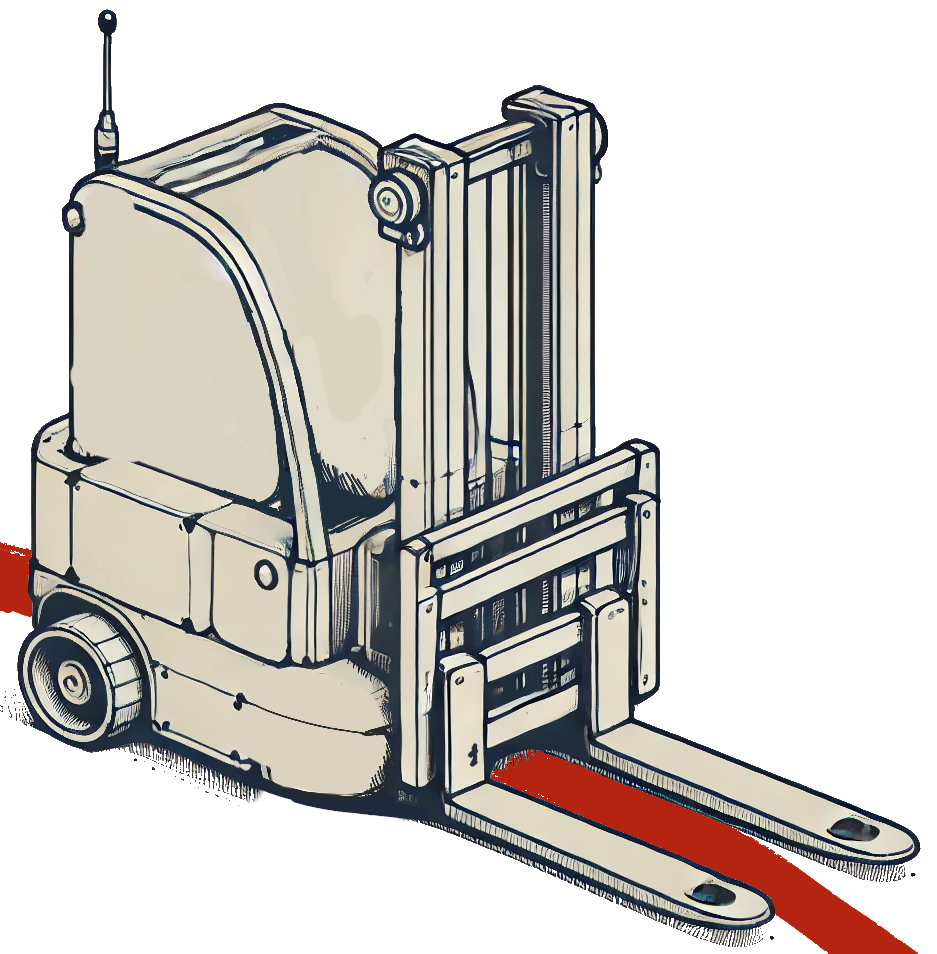
\includegraphics[width=\textwidth]{Simple_sketch_of_an_automated_forklift_robot_with_two_wheels_at_the_back_and_one_wheel_in_the_front.png}
        \caption{Three wheel line following design}
        \label{fig:three_wheel_line_flowing}
    \end{minipage}
    \hfill
    \begin{minipage}{0.48\textwidth}
        \centering
        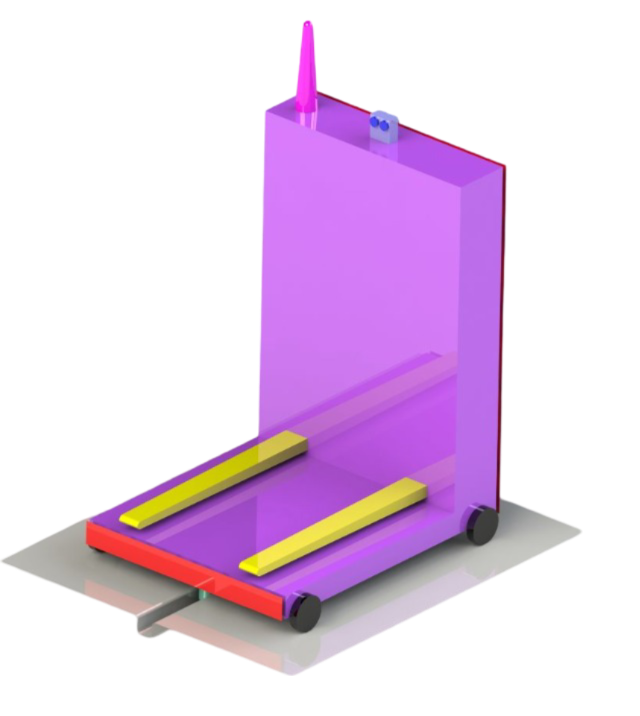
\includegraphics[width=\textwidth]{anna&will's design (1).png}
        \caption{Four wheel monorail design}
        \label{fig:design_idea}
    \end{minipage}
\end{figure}

\begin{figure}[h!]
    \centering
    \begin{minipage}{0.48\textwidth}

        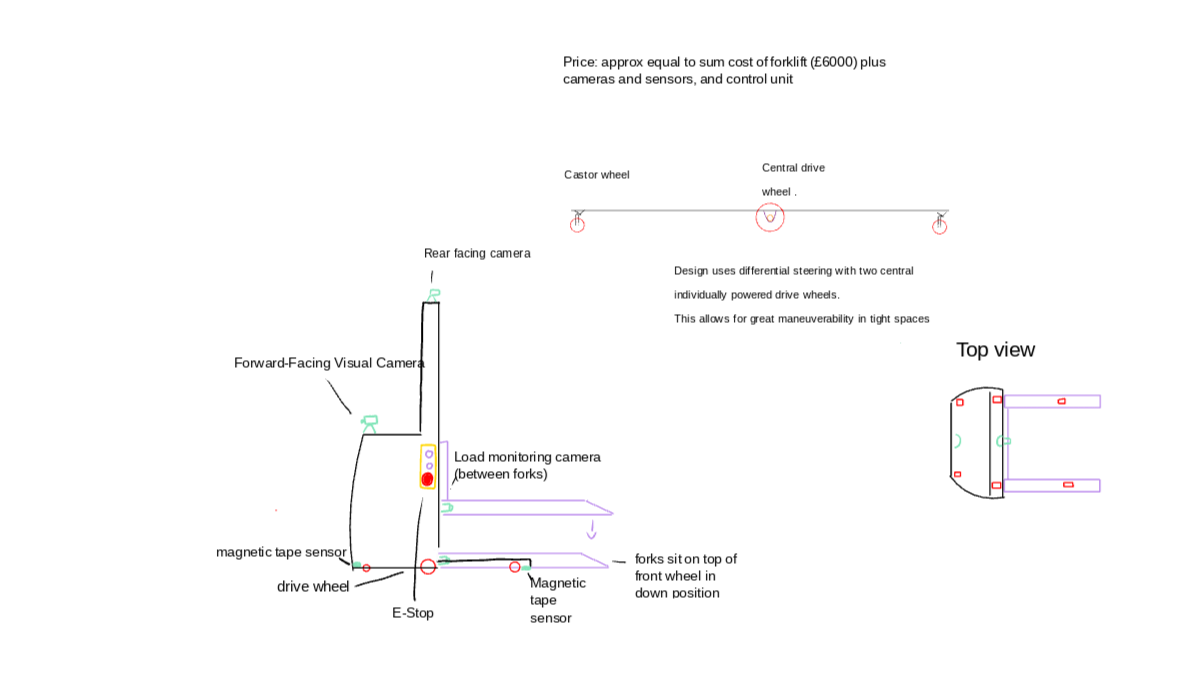
\includegraphics[width=1\textwidth]{Louis's design.png}
        \caption{Six wheel line following design}
        \label{fig:louis_design}
    \end{minipage}
    \hfill
    \begin{minipage}{0.48\textwidth}
      
        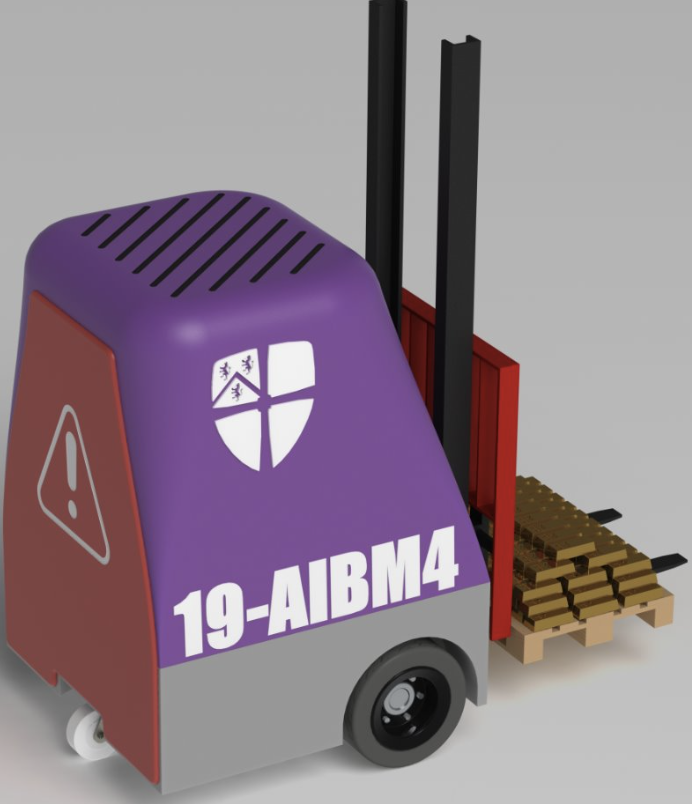
\includegraphics[width=\textwidth]{finaldesign1.png}
        \caption{Final design}
        \label{fig:final_design}
    \end{minipage}
\end{figure}


\end{enumerate}

\subsection{Strengths and Weaknesses}
Each concept was evaluated against the URS. A summary of strengths and weaknesses is provided in Table \ref{tab:concept_evaluation}.


\begin{table}[h!]
\centering
\caption{Concept Evaluation Matrix}
\begin{tabular}{@{}lcc@{}}
\toprule
\textbf{Criteria}      & \textbf{Concept 1} & \textbf{Concept 2} \\ \midrule
Load Capacity          & High               & Medium             \\
Navigation Efficiency  & Medium             & High               \\
Cost                   & Low                & Medium             \\
Ease of Maintenance    & High               & Low                \\ \bottomrule
\end{tabular}
\label{tab:concept_evaluation}
\end{table}

% -------------------------------------------------------------
% 4. Chosen Solution(s)
% -------------------------------------------------------------
\section{Chosen Solution(s)}

\subsection{Proposed Solution}
The three-wheeled heavy-duty material mover, is chosen due to its balance of cost, efficiency, and reliability. 
The body and forks are likely to be made from steel because it has the highest recycling rate among all materials used in construction and engineering  \cite{baker2023}
The drive wheels.  

\subsection{Expected Cost}



{The estimated cost of the product \cite{P. Hinz} is £60,000, and this covers:}
\begin{itemize}
    \item All the hardware for the autonomous material mover and its implementation into the factory.
    \item All of the software acquisition and development for navigation, obstacle detection, and task automation.
    \item The implementation of the system into a conventional factory; however, this will likely differ on a site-to-site basis.
\end{itemize}


\begin{table}[h!]
    \centering
    \begin{tabular}{|l|r|}
        \hline
        \textbf{Cost Item}          & \textbf{Amount (£)} \\ \hline
        Labour Costs                 & 18,000.00           \\ \hline
        Material Costs              & 15,099.12           \\ \hline
        Overheads                   & 10,000.00           \\ \hline
        Software and Simulation     & 2,000.00            \\ \hline
        Contingency                 & 4,900.88            \\ \hline
        \textbf{Total Estimated Cost} & \textbf{60,000.00}  \\ \hline
    \end{tabular}
    \caption{Breakdown of Expected Costs for the Autonomous Material Mover}
    \label{tab:expected_costs}
\end{table}
\FloatBarrier
\subsection{Cost Comparison for a Customer}
Whilst this product may seem expensive at first to potential customers, it has distinct financial and logistical advantages over manual forklifts. A 2-ton manual stacker truck can cost anywhere from £8000 for a standing operator push model, to £25000 for a full truck. In addition to the cost of the stacker there is the cost of paying operators. 
This soon adds up, with hourly minimum wage in the UK being £11.44, this being the largest factor in running costs. An automated stacker eliminates this expense, whilst also being able to work continuously with only breaks for charging.

It should be considered that automated forklifts do on average move slower than regular manually driven forklifts. This means that it takes around 1.3-1.5 automated forklifts to do the same work as a single manned truck \cite{Pastor-Tella2024}. 
Taking these things into consideration, the following table assumes a factory using two manned forklifts, and how these costs would compare to three AGVs.
\begin{figure}[h!]
    \centering
     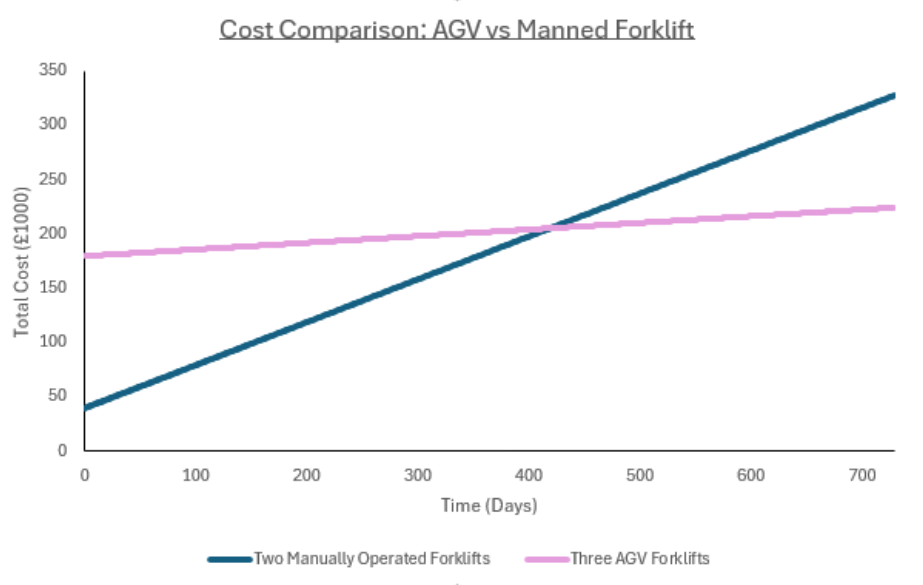
\includegraphics[width=1\textwidth]{CostComparisonGraphUpdatedV2.png}
        \caption{Cost Comparison: AGVs vs Manned Forklifts}
         \label{fig:timeline}
\end{figure}
\FloatBarrier
Cost per unit taken as £60,000 for an AGV, compared with £20,000 for a manual forklift. From the graph we can see that after 420 days of operation the three AGV forklifts become more economical in comparison to the two manually operated forklifts.



 

\section*{Breakeven Analysis: AGVs vs. Manual Forklifts}

 \begin{itemize}
    \item \( C_0 \): Total Initial Cost (purchase, installation, training.)
    \item \( C_1 \): Annual Operating Costs (maintenance, energy, insurance.)
    \item \( S \): Annual Savings (labor cost savings)
    \item \( T_{\text{breakeven}} \): Breakeven Period (in years)
\end{itemize}

\section{Step 5: Return on Investment (ROI)}
To calculate the Return on Investment (ROI) after the breakeven period 
\[
\text{ROI} = \frac{S \times (T - T_{\text{breakeven}})}{C_0} \times 100
\]
 
\begin{table}[htbp]
\centering
\begin{tabular}{|l|l|l|}
\hline
\textbf{Cost Factor}                   & \textbf{Manual Forklifts}           & \textbf{AGVs } \\ \hline
\textbf{Initial Cost per Unit}          & £20,000                             & £60,000                               \\ \hline
\textbf{Number of Units}                & 2                                    & 3                                     \\ \hline
\textbf{Total Initial Cost}             & 2 × £20,000 = £40,000               & £180,000                \\ \hline
\textbf{Annual labour cost per forklift }& £11.07× 16×365 = £64,648.80      & £0                                    \\ \hline
\textbf{Total Annual Labor Cost (16 hours a day)}        & £129,297.6    & £0                                    \\ \hline
 \textbf{Electricity cost per year (25.46p per kWh) }& £14,868&£22,302\\\hline  
 
\textbf{Total Annual Operating Cost}    & £144,165& £22,302\\ \hline
 
  
\end{tabular}

\caption{Cost Breakdown for Automated Forklifts}
\end{table}



 (assuming )


 \begin{figure}[h!]
    \centering
    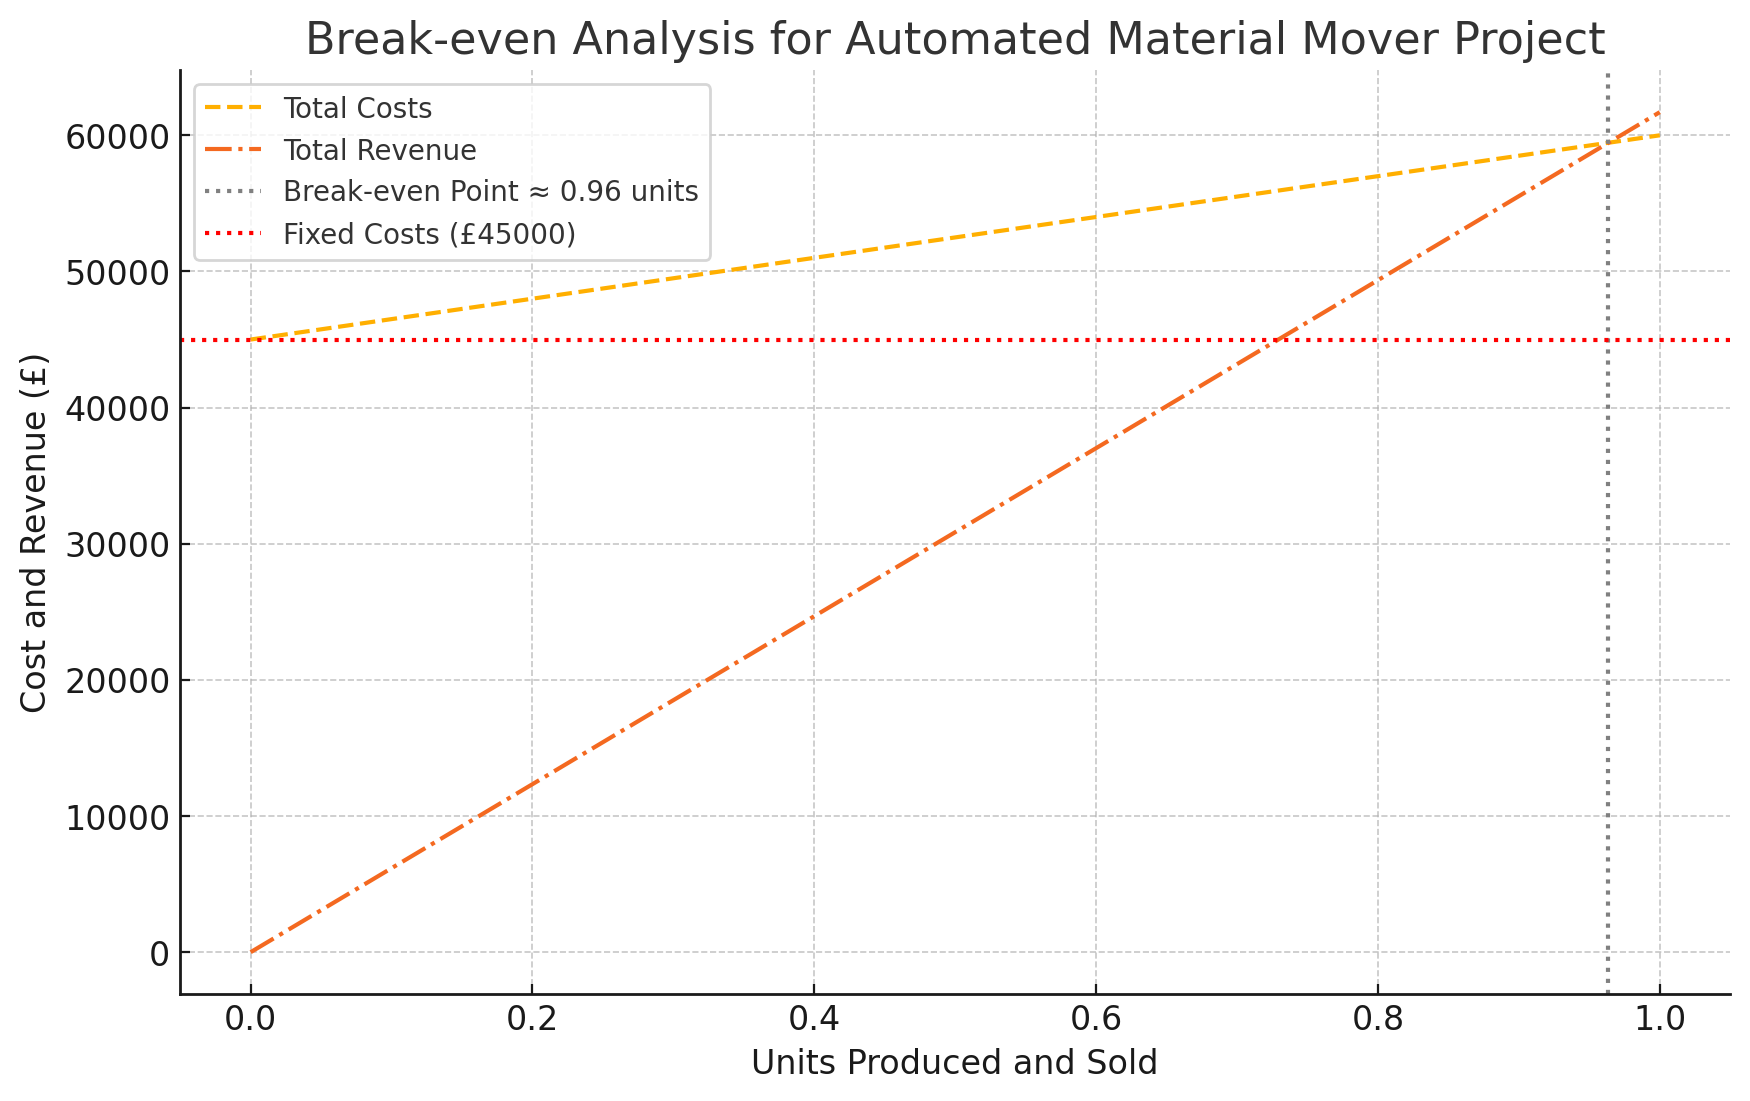
\includegraphics[width=1\textwidth]{breakeven.png}  % Adjust width as needed
    \caption{Breakeven Point Analysis}
    \label{fig:breakeven}
\end{figure} 

 

\subsection*{Breakeven Calculation (with Labor Savings)}

 

 
 

 
 

\subsection*{Breakeven Point Plot}

  


\subsection{Factory design}

\begin{figure}[ht]
\centering
\begin{minipage}{0.45\textwidth}
    \centering
    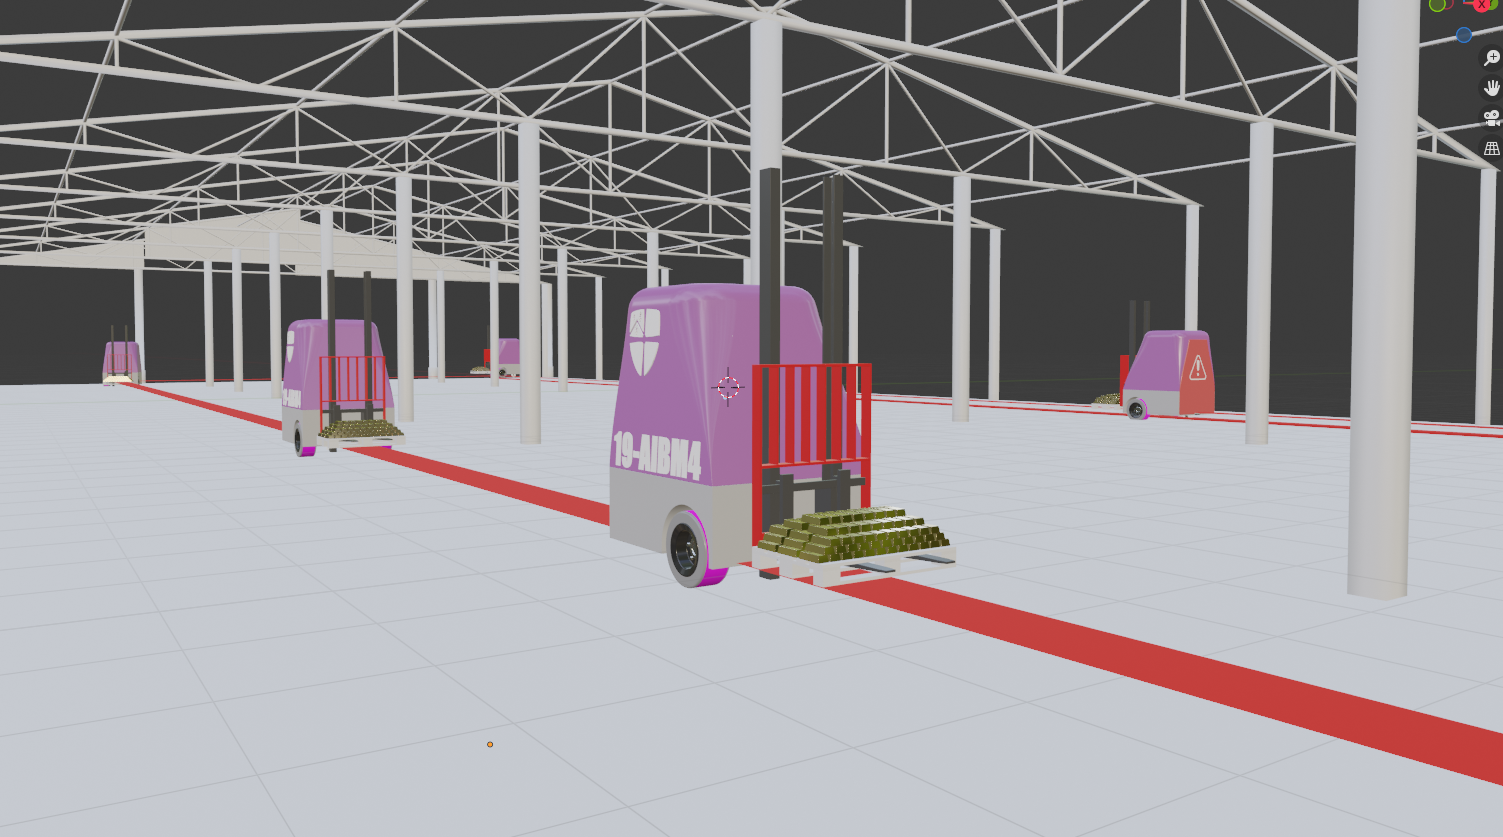
\includegraphics[width=\linewidth]{factory layout1.png}
    \caption{Factory design}
    \label{fig:targeted working condition}
\end{minipage}%
\hfill
\begin{minipage}{0.45\textwidth}
    \centering
    \begin{tabular}{|l|l|}
    \hline
    \textbf{Dimension}      & \textbf{Value}                \\ \hline
    \textbf{Floor Area}      & 10,628 sq ft (989.8 m²)        \\ \hline
    \textbf{Eaves Height}    & 6 meters (19.7 feet)           \\ \hline
    \textbf{Width}           & ~100 feet (30.5 meters)        \\ \hline
    \textbf{Length}          & ~106 feet (32.3 meters)        \\ \hline
    \end{tabular}
    \caption{ Dimensions for Unit 5, Aycliffe Business Park\cite{mileway_hurworth_2024}}
\end{minipage}
\end{figure}



Based on the information from the EG Propertylink listing for Unit 5, Hurworth Road, Aycliffe Business Park\cite{mileway_hurworth_2024}, the CAD factory layout design integrates the key features and constraints of the property.  Line-following forklifts rely on predefined paths marked by visible or magnetic lines (often in the form of tape or sensors) on the floor, the layout was optimized to include narrower aisles suitable for line-following AGVs,  ensuring they have sufficient room to follow the lines without obstruction which take full advantage of the 6-meter eaves height . 

Clearly defined line-following paths throughout the facility marked with high-visibility lines (magnetic strips), guide the forklifts through the warehouse, directing them to storage zones, picking locations, and loading bays.A dedicated area for charging stations was incorporated into the layout . Automated docking stations be strategically located near the production and storage zones, ensuring AGVs can easily return to their charging points without disrupting material handling operations. 

 
 \section{Risk assessment }
 
\begin{figure}[h!]
    \centering
    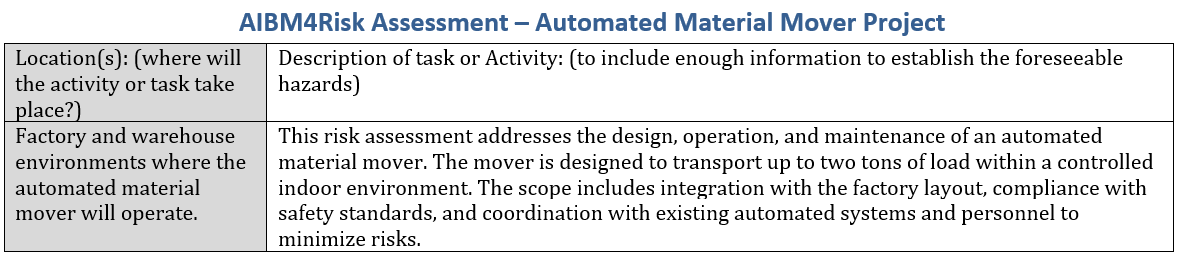
\includegraphics[width=0.85\textwidth]{Risk1.png}
    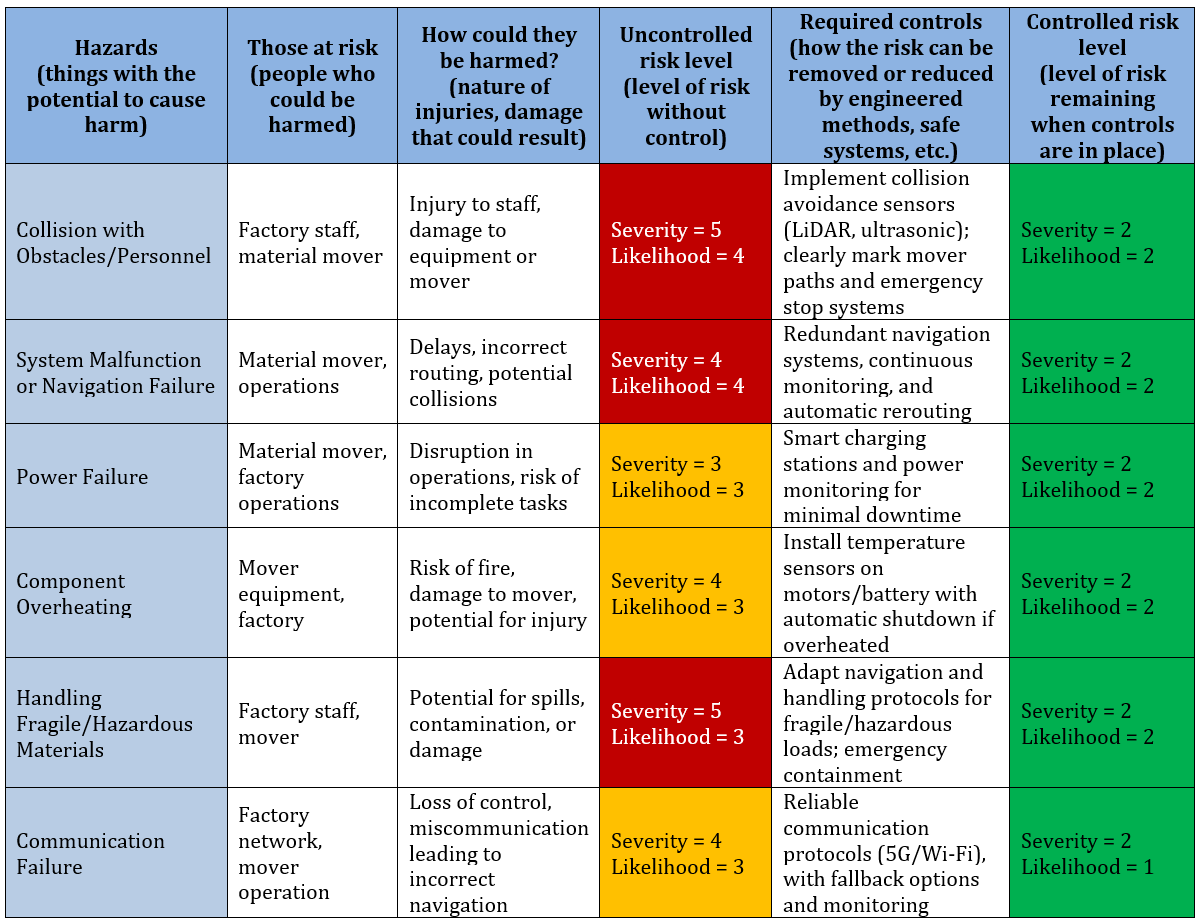
\includegraphics[width=0.85\textwidth]{Risk2.png}
    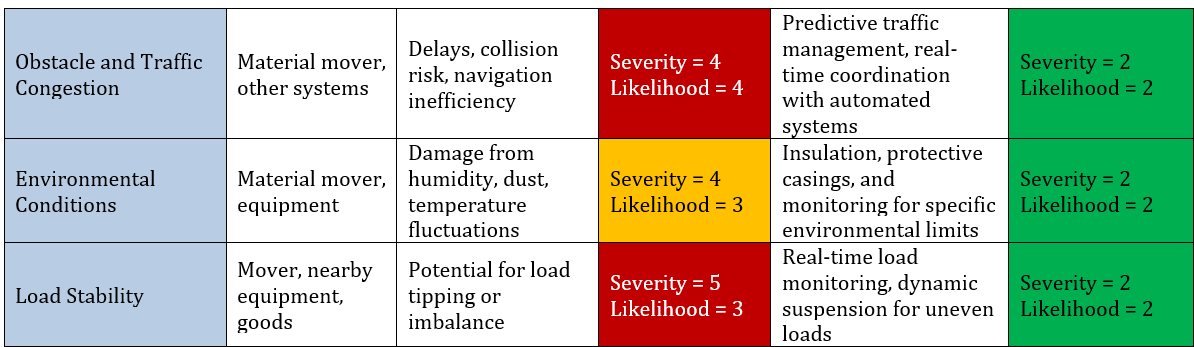
\includegraphics[width=0.85\textwidth]{Risk3.png}
    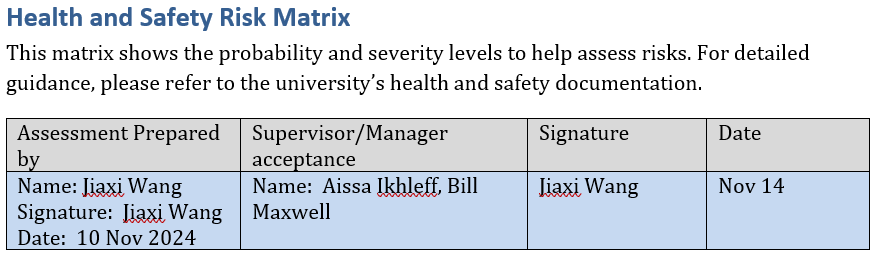
\includegraphics[width=0.85\textwidth]{Risk4.png}
    \caption{Risk Assessment – Automated Material Mover Project}
    \label{fig:risk_assessment}
\end{figure}
\FloatBarrier


% -------------------------------------------------------------
% 5. Recommendations / Conclusions
% -------------------------------------------------------------
\section{Recommendations / Conclusions}
\begin{itemize}
    \item Modify the URS to include advanced collision-avoidance features.
    \item Proceed with the development of the four-wheeled design.
    \item The project has high feasibility, promising an ROI within 2 years.
\end{itemize}


% -------------------------------------------------------------
% 6. Project Schedule
% -------------------------------------------------------------
\section{Project Schedule}
\subsection{Gantt Chart}
In order to plan out the schedule throughout the project, a Gantt Chart was created to plan out the hours worked every week, working around holidays and other module deadlines. This ensures no tasks are ignored or missed out, giving them ample time to be completed. Additionally, leaving contingency hours caters for scope creep and any drastic changes that need to be made and also giving flexibility to change tasks and the hours put into them. 

    The dynamic Gantt Chart in \hl{Figure X}, made using Microsoft Excel, shows how complete each task is, and helps to visualise which tasks are on track, ahead or behind schedule. 
\begin{figure}[h!]
    \centering
    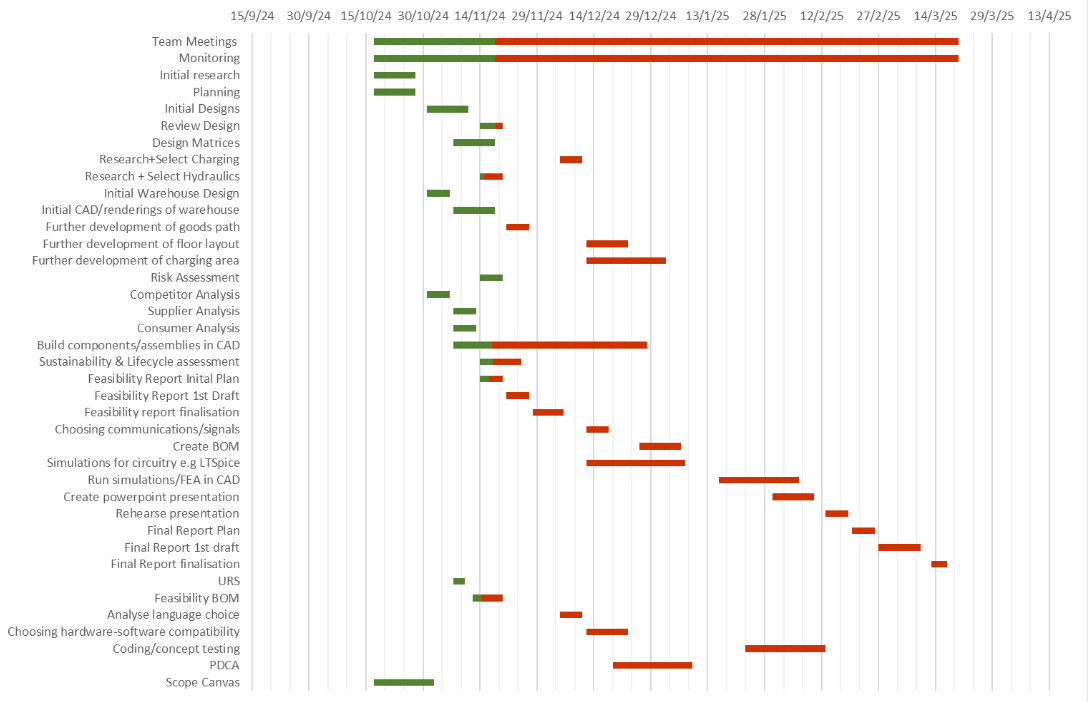
\includegraphics[width=0.9\textwidth]{dynamicganttchart.png}
    \caption{Dynamic Project Gantt Chart}
    \label{fig:x}
\end{figure}

The planning Gantt Chart, \hl{Figure Y}, showcases the weekly hours expected to be put into tasks and helps to ensure a balanced workload throughout the project. It also allows foresight for deadlines and other departmental commitments so that the workload can be planned around these accordingly. As shown in the Gantt Chart below, the majority of first term was planned around choosing a feasible design for the material mover and the research and drawings for this, as well as the factory layout the mover would work in. This provides a strong basis for the remainder of the project which focuses on CAD, software proof of concept and other simulations. This plan also allows for scope creep, having 135 contingency hours, and so means the project has ample time to be complete before the Final Project Report.
\begin{figure}
    \centering
    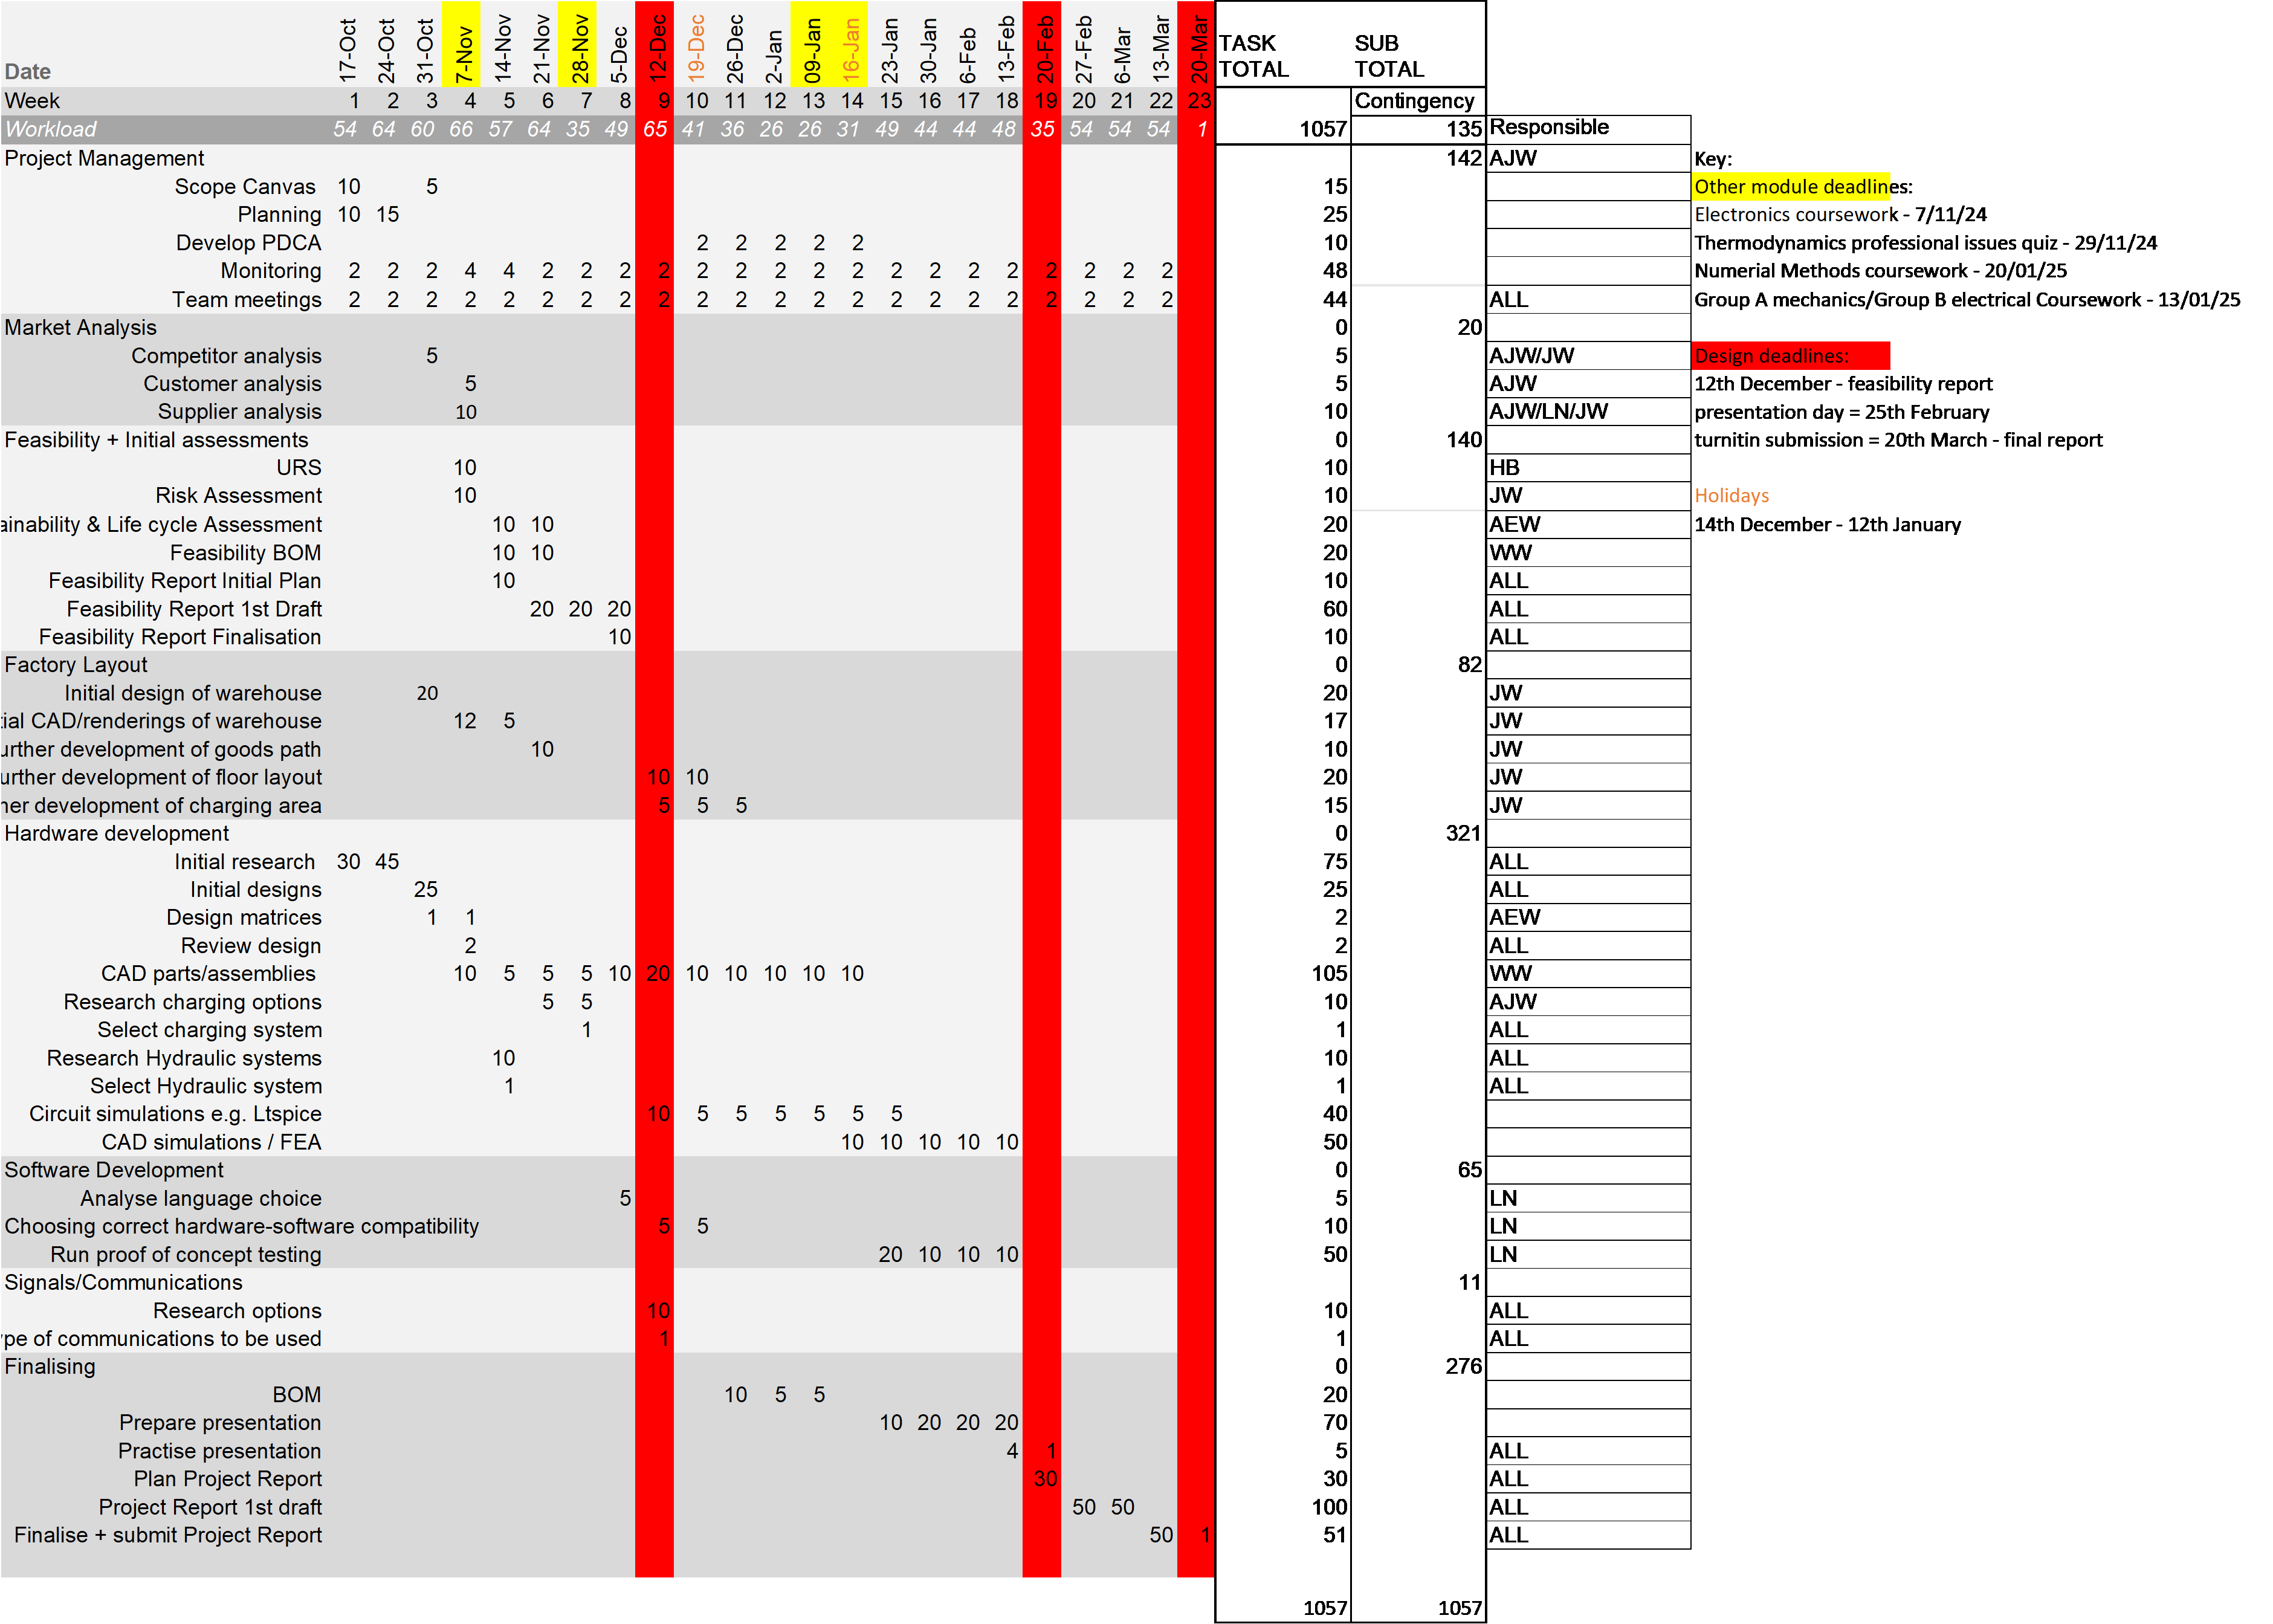
\includegraphics[width=0.9\linewidth]{even bigger gantt chart.png}
    \caption{Planning Gantt Chart}
    \label{fig:y}
\end{figure}
\subsection{Meeting Minutes}
% -------------------------------------------------------------
% 7. References
% -------------------------------------------------------------

 \newpage
%\bibliographystyle{unsrt}
%\bibliography{reference}


\begin{thebibliography}{99}

\bibitem{MathWorks}
MathWorks, “What Is SLAM (Simultaneous Localization and Mapping) – MATLAB \& Simulink,” \textit{uk.mathworks.com}.  
Available at: \url{https://uk.mathworks.com/discovery/slam.html} (accessed Nov. 20, 2024).
 

\bibitem{ToyotaForklifts}
Toyota Forklifts, “Automated Warehouse Trucks,” \textit{toyota-forklifts.co.uk}.  
Available at: \url{https://toyota-forklifts.co.uk/automated-solutions/automated-warehouse-trucks/} (accessed Nov. 20, 2024).

\bibitem{Forkify}
Forkify, “Forklift Cost Buyers Guide,” \textit{forkify.com}.  
Available at: \url{https://forkify.com/buyers-guide/forklift-cost/} (accessed Nov. 20, 2024).


\bibitem{LangleyShop}
Langley Shop, “Forklift Forks 100x40x1200 Class 2A,” \textit{langleyshop.co.uk}.  
Available at: \url{https://www.langleyshop.co.uk/product/forklift-forks-100x40x1200-class-2a/} (accessed Nov. 20, 2024).

\bibitem{CheckaTrade}
Checkatrade, “Electric Car Charger Installation Cost,” \textit{checkatrade.com}.  
Available at: \url{https://www.checkatrade.com/blog/cost-guides/electric-car-charger-installation-cost/} (accessed Nov. 20, 2024).

\bibitem{SalaryExpert}
Salary Expert, “Forklift Driver Salary in South Korea,” \textit{salaryexpert.com}.  
Available at: \url{https://www.salaryexpert.com/salary/job/forklift-driver/south-korea?form=MG0AV3} (accessed Nov. 20, 2024).

\bibitem{MordorIntelligence}
Mordor Intelligence, “Automated Material Handling Market,” \textit{mordorintelligence.com}.  
Available at: \url{https://www.mordorintelligence.com/industry-reports/automated-material-handling-market} (accessed Nov. 20, 2024).

\bibitem{GrandViewResearch}
Grand View Research, “Automated Guided Vehicle (AGV) Market,” \textit{grandviewresearch.com}.  
Available at: \url{https://www.grandviewresearch.com/industry-analysis/automated-guided-vehicle-agv-market} (accessed Nov. 20, 2024).

\bibitem{baker2023} T. Baker, ``5 Reason Why Structural Steel is Such a Sustainable Material,'' \textit{Baker Steel Trading}, 2023. [Online]. Available: \url{https://www.bakersteeltrading.co.uk/is-structural-steel-sustainable/}. [Accessed: Nov. 21, 2024].

\bibitem{eco2022} S. Co, ``We use ECO-FRIENDLY production techniques and technology,'' \textit{ENJOYING GO}, Sep. 21, 2022. [Online]. Available: \url{https://www.enjoycaster.com/en/solutions/product/eco-friendly-production}. [Accessed: Nov. 25, 2024].

\bibitem{brake2021} ``The Future Of Tires: Sustainable, Airless \& Connected,'' \textit{Brake \& Front End}, 2021. [Online]. Available: \url{https://www.brakeandfrontend.com/the-future-of-tires-sustainable-airless-connected/}. [Accessed: Nov. 21, 2024].


\bibitem{roos2012} D. Roos, ``5 Green Methods of Transporting Goods,'' \textit{HowStuffWorks}, Aug. 29, 2012. [Online]. Available: \url{https://science.howstuffworks.com/environmental/green-science/5-green-methods-transporting-goods.htm}. [Accessed: Nov. 25, 2024].

\bibitem{ashmore2024} J. Ashmore, ``Container Operator BG Freight Line Launches Greenest Newbuild Vessels to Drive Sustainability,'' \textit{Afloat.ie}, May 08, 2024. [Online]. Available: \url{https://afloat.ie/port-news/port-and-shipping-news/item/63086-bg-freight-line-launches-new-vessels-to-drive-sustainability}. [Accessed: Nov. 25, 2024].


\bibitem{P. Hinz}
P. Hinz, “How Much Electricity does a Forklift Use per Hour?,” Adaptalift, Sep. 2021. \url{https://www.adaptalift.com.au/blog/how-much-electricity-does-a-forklift-use-per-hour }(accessed Nov. 25, 2024).

 \bibitem{mileway_hurworth_2024}
Mileway, “Hurworth Road, Newton Aycliffe Industrial Estate,” \url{https://mileway.com/properties/gb/portfolio/hurworth-road-newton-aycliffe-industrial-estate/} (accessed Dec. 2, 2024).

 \bibitem{Pastor-Tella2024}
A. Pastor-Tella, "AGV Cost Whitepaper" 



\bibitem{crown2024}

Crown Equipment Corporation, \textit{Achieving Sustained Automated Forklift Performance}, 2024, \url{https://www.crown.com/en-us/blog/articles/automation/Achieving-Sustained-Automated-Forklift-Performance.html#:~:text=Fortunately%2C%20automated%20forklifts%20require%20much,on%20and%20within%20the%20vehicle.} (Accessed: December 2, 2024).


% -------------------------------------------------------------

% -------------------------------------------------------------
% BIBLIOGRAPHY (LOCAL) - Uncomment to use instead of BIB
% ------------------------------------------------------------
 

\end{thebibliography}
 

% Start bibliography
% %                                                             % Can be in a separate file, \input(...)
                      % Author names
%         Plastic deformation of cellular materials,                                  % Title of publication
%         \textit{Reference Module in Materials Science and Materials Engineering},   % Journal name
%         2016.                                                                       % Vol, num, pg, year
% %
% \bibitem{Lee:2017aa} J.H. Lee, D.R. Howel, W.P. Meehan III, G.L. Iverson, A.J. Gardner.
%         Effects of Exercise on Sport Concussion Assessment Tool--Third Edition Performance in Professional Athletes,
%         \textit{The Orthopaedic Journal of Sports Medicine},
%         \textbf{5}(9):1--7, 2017. 
% %
% \bibitem{Lang:1988aa} R.J. Lang.
%         \textit{The complete book of origami: Step-by-step instructions in over 1000 diagrams},
%         Dover Publications, Inc.
%         1988. 
% %
% \bibitem{Kingslake:1992aa} R. Kingslake.
%         \textit{Optics in photography},
%         SPIE Optical engineering press
%         1992. 
% %
% \bibitem{Chen:2011ab} W. Chen, B. Song.
%         \textit{Split Hopkinson (Kolsky) bar: Design, Testing and Applications},
%         Mechanical Engineering Series, Springer
%         2011. 
% %
% \bibitem{Fairlie:2008aa} G.E. Fairlie, R. Hart, E.J. Draper.
%         \textit{Structural response to high explosive blast loading},
%         in MABS 20 - Military Aspects of Blast and Shock,
%         2008. 
% %
                                      % End bibliography

% -------------------------------------------------------------
% LISTS OF FIGURES AND TABLES
% -------------------------------------------------------------
\section{Appendices}
\listoffigures                                                % Add list of figures
\listoftables                                                 % Add list of tables

% -------------------------------------------------------------
% WORD COUNT OUTPUT


% 8. Appendices
% -------------------------------------------------------------

\hl{Additional charts, data, or images can be included here.}

\end{document}
